% Options for packages loaded elsewhere
\PassOptionsToPackage{unicode}{hyperref}
\PassOptionsToPackage{hyphens}{url}
%
\documentclass[
  english,
  ,jou,floatsintext]{apa6}
\usepackage{lmodern}
\usepackage{amssymb,amsmath}
\usepackage{ifxetex,ifluatex}
\ifnum 0\ifxetex 1\fi\ifluatex 1\fi=0 % if pdftex
  \usepackage[T1]{fontenc}
  \usepackage[utf8]{inputenc}
  \usepackage{textcomp} % provide euro and other symbols
\else % if luatex or xetex
  \usepackage{unicode-math}
  \defaultfontfeatures{Scale=MatchLowercase}
  \defaultfontfeatures[\rmfamily]{Ligatures=TeX,Scale=1}
\fi
% Use upquote if available, for straight quotes in verbatim environments
\IfFileExists{upquote.sty}{\usepackage{upquote}}{}
\IfFileExists{microtype.sty}{% use microtype if available
  \usepackage[]{microtype}
  \UseMicrotypeSet[protrusion]{basicmath} % disable protrusion for tt fonts
}{}
\makeatletter
\@ifundefined{KOMAClassName}{% if non-KOMA class
  \IfFileExists{parskip.sty}{%
    \usepackage{parskip}
  }{% else
    \setlength{\parindent}{0pt}
    \setlength{\parskip}{6pt plus 2pt minus 1pt}}
}{% if KOMA class
  \KOMAoptions{parskip=half}}
\makeatother
\usepackage{xcolor}
\IfFileExists{xurl.sty}{\usepackage{xurl}}{} % add URL line breaks if available
\IfFileExists{bookmark.sty}{\usepackage{bookmark}}{\usepackage{hyperref}}
\hypersetup{
  pdftitle={Integrating analysis code and document preparation : A minimal example Rmarkdown + papaja document},
  pdfauthor={Tom Stafford1 \& Able Coauthor2},
  pdflang={en-EN},
  hidelinks,
  pdfcreator={LaTeX via pandoc}}
\urlstyle{same} % disable monospaced font for URLs
\usepackage{graphicx,grffile}
\makeatletter
\def\maxwidth{\ifdim\Gin@nat@width>\linewidth\linewidth\else\Gin@nat@width\fi}
\def\maxheight{\ifdim\Gin@nat@height>\textheight\textheight\else\Gin@nat@height\fi}
\makeatother
% Scale images if necessary, so that they will not overflow the page
% margins by default, and it is still possible to overwrite the defaults
% using explicit options in \includegraphics[width, height, ...]{}
\setkeys{Gin}{width=\maxwidth,height=\maxheight,keepaspectratio}
% Set default figure placement to htbp
\makeatletter
\def\fps@figure{htbp}
\makeatother
\setlength{\emergencystretch}{3em} % prevent overfull lines
\providecommand{\tightlist}{%
  \setlength{\itemsep}{0pt}\setlength{\parskip}{0pt}}
\setcounter{secnumdepth}{-\maxdimen} % remove section numbering
% Make \paragraph and \subparagraph free-standing
\ifx\paragraph\undefined\else
  \let\oldparagraph\paragraph
  \renewcommand{\paragraph}[1]{\oldparagraph{#1}\mbox{}}
\fi
\ifx\subparagraph\undefined\else
  \let\oldsubparagraph\subparagraph
  \renewcommand{\subparagraph}[1]{\oldsubparagraph{#1}\mbox{}}
\fi
% Manuscript styling
\usepackage{upgreek}
\captionsetup{font=singlespacing,justification=justified}

% Table formatting
\usepackage{longtable}
\usepackage{lscape}
% \usepackage[counterclockwise]{rotating}   % Landscape page setup for large tables
\usepackage{multirow}		% Table styling
\usepackage{tabularx}		% Control Column width
\usepackage[flushleft]{threeparttable}	% Allows for three part tables with a specified notes section
\usepackage{threeparttablex}            % Lets threeparttable work with longtable

% Create new environments so endfloat can handle them
% \newenvironment{ltable}
%   {\begin{landscape}\begin{center}\begin{threeparttable}}
%   {\end{threeparttable}\end{center}\end{landscape}}
\newenvironment{lltable}{\begin{landscape}\begin{center}\begin{ThreePartTable}}{\end{ThreePartTable}\end{center}\end{landscape}}

% Enables adjusting longtable caption width to table width
% Solution found at http://golatex.de/longtable-mit-caption-so-breit-wie-die-tabelle-t15767.html
\makeatletter
\newcommand\LastLTentrywidth{1em}
\newlength\longtablewidth
\setlength{\longtablewidth}{1in}
\newcommand{\getlongtablewidth}{\begingroup \ifcsname LT@\roman{LT@tables}\endcsname \global\longtablewidth=0pt \renewcommand{\LT@entry}[2]{\global\advance\longtablewidth by ##2\relax\gdef\LastLTentrywidth{##2}}\@nameuse{LT@\roman{LT@tables}} \fi \endgroup}

% \setlength{\parindent}{0.5in}
% \setlength{\parskip}{0pt plus 0pt minus 0pt}

% \usepackage{etoolbox}
\makeatletter
\patchcmd{\HyOrg@maketitle}
  {\section{\normalfont\normalsize\abstractname}}
  {\section*{\normalfont\normalsize\abstractname}}
  {}{\typeout{Failed to patch abstract.}}
\patchcmd{\HyOrg@maketitle}
  {\section{\protect\normalfont{\@title}}}
  {\section*{\protect\normalfont{\@title}}}
  {}{\typeout{Failed to patch title.}}
\makeatother
\shorttitle{Example Rmarkdown document}
\usepackage{dblfloatfix}


\usepackage{csquotes}
\ifxetex
  % Load polyglossia as late as possible: uses bidi with RTL langages (e.g. Hebrew, Arabic)
  \usepackage{polyglossia}
  \setmainlanguage[]{english}
\else
  \usepackage[shorthands=off,main=english]{babel}
\fi

\title{Integrating analysis code and document preparation : A minimal example Rmarkdown + papaja document}
\author{Tom Stafford\textsuperscript{1} \& Able Coauthor\textsuperscript{2}}
\date{}


\note{\textcolor{red}{This is an example of a note}}

\affiliation{\vspace{0.5cm}\textsuperscript{1} Department of Psychology, University of Sheffield\\\textsuperscript{2} Department of Psychosocial Science, University of Bergen}

\abstract{
R is a statistical programming language which is increasingly popular with psychologists. It can import and process your data, fit statistical models (from simple t-tests to state of the art such as bayesian multilevel model fitting). It also makes nice plots. RStudio is a way of editing R scripts and running R analysis. RMarkdown is a way of using RStudio to produce documents (e.g.~as webpages, MS Word or PDF). Another advantage is that you can include R code in your document file - so no more running your analysis in SPSS and copying the results into your document (and making errors / forgetting which version of the analysis you ran etc). This is an example document which integrates all the functions of Rmarkdown - running analysis, formatting references, etc. It uses an add-on for Rmarkdown called papaja which helps us make nicely APA formatted documents
}



\begin{document}
\maketitle

\hypertarget{introduction}{%
\section{Introduction}\label{introduction}}

You will find it useful to compare the output PDF document with the .rmd document. This latter item is the thing you edit to produce the PDF.

\hypertarget{example-subheading}{%
\subsection{Example Subheading}\label{example-subheading}}

Here are some example references in the following sentence. For reviews of this topic see Wickelgren (1977); Heitz (2014). Here is another example reference (e.g.~Stafford, Pirrone, Croucher, \& Krystalli, 2020)\footnote{As well as an example of a footnote.}. This paper was produced as part of the \enquote{code club} held in the Department of Psychology at the Univetrsity of Sheffield in 2019, organised by Tom Stafford and Kat Giannadou.

\hypertarget{method}{%
\section{Method}\label{method}}

Rmarkdown also lets us track figure labels, and updates them automatically. Look! Kittens! Illustrated in Figure \ref{fig:examplefigurename}.

\begin{figure}

{\centering 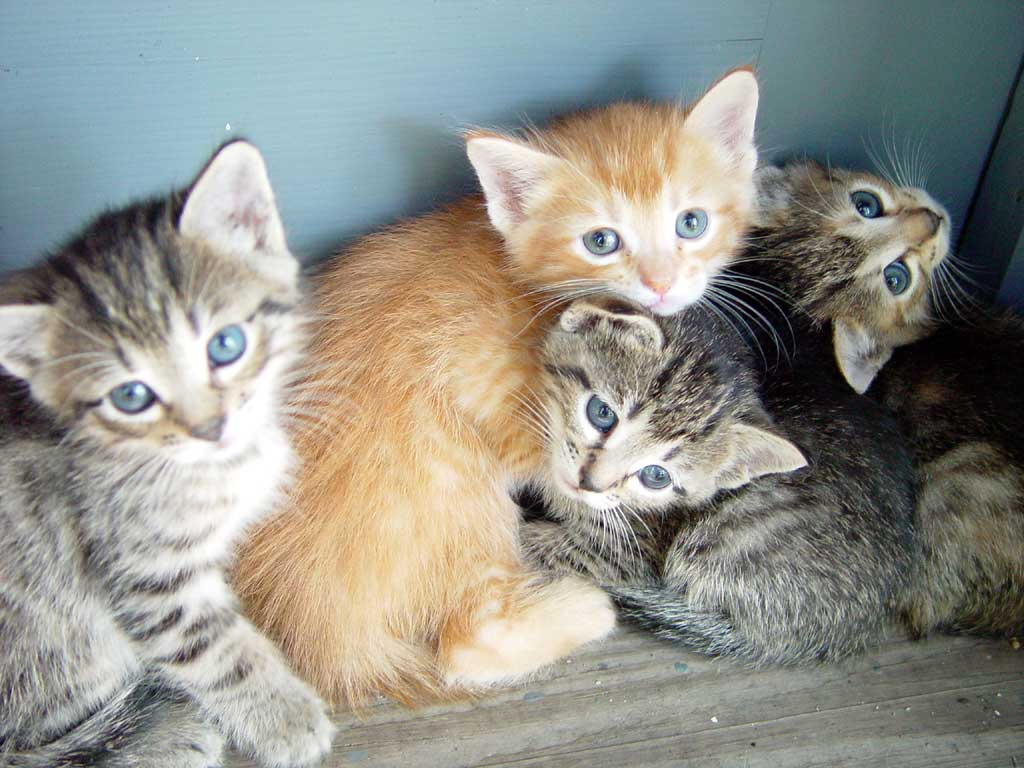
\includegraphics[width=0.75\linewidth]{figs/kittens} 

}

\caption{Example figure caption}\label{fig:examplefigurename}
\end{figure}

\hypertarget{requirements}{%
\subsection{Requirements}\label{requirements}}

You should install R, RStudio and tex and papaja (Aust \& Barth, 2020). More details here \url{https://crsh.github.io/papaja_man/introduction.html\#getting-started}

\hypertarget{results}{%
\section{Results}\label{results}}

Now let's integrate some R code to generate/import some data, run and analyse and integrate it into the document:

You can't see it, but in between this paragraph and the last we asked R to generate some random data and save it to a CSV file. Now we're going to import the data from the CSV file, as if it was independently created data - from an experiment or similar - and plot a graph.

\begin{figure}

{\centering 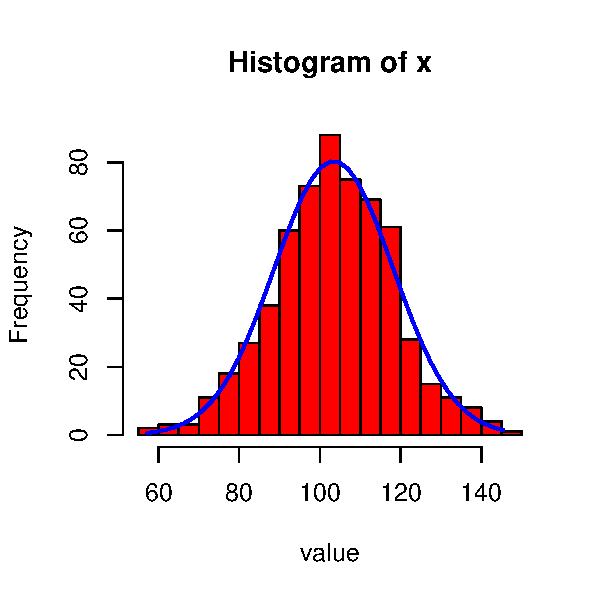
\includegraphics[width=0.75\linewidth]{example_manuscript_files/figure-latex/ourhistogram-1} 

}

\caption{Histogram of all data, grouped}\label{fig:ourhistogram}
\end{figure}

See Figure \ref{fig:ourhistogram}. Of course we could draw all sorts of things, but this is a proof-of-concept. Finally, let's run a t-test and integrate the results into the text.

We found there was a statistically significant difference between the two groups (t=-6.33 (591.15), p = 0.00). Note how the exact values in the previous sentence change every time we re-make the document (because the document also re-generates the underlying data).

Unanswered questions: Is this the best way to integrate values into text? Why is the df not an integer? What is the best way to define figure sizes so you get nice and/or consistent sizing across document formats?

\hypertarget{discussion}{%
\section{Discussion}\label{discussion}}

Make your document by opening .Rmd file in RStudio and clicking \enquote{knit}

Rmarkdown is good (Allaire et al., 2020). Need to change reference style? Change one line. Need to submit as PDF rather than .DOC? Just click \enquote{Word} as output rather than \enquote{PDF} (instructions here \url{https://rmarkdown.rstudio.com/articles_docx.html}). Need to change to two column style to make a nice pre-print? Again, simple - just change one line! In line 40 \enquote{class : \enquote{man}} gives you manuscript style; \enquote{jou} gives you two column style.

To port to your own project just copy across these files:

\begin{itemize}
\tightlist
\item
  example\_manuscript.rmd
\item
  apa6.cls - style file which makes everything look APA format nice
\item
  references.bib - information on references in bibtex format
\item
  figs folder - where images integrated into the manuscript are kept
\end{itemize}

\hypertarget{main-conclusions}{%
\subsection{Main conclusions}\label{main-conclusions}}

Of course, there's more effort in installing and learning and correctly marking up your document in the first place, but it is worth it

\hypertarget{acknowledgements}{%
\section{Acknowledgements}\label{acknowledgements}}

This is an example acknowledgments section.

\hypertarget{references}{%
\section*{References}\label{references}}
\addcontentsline{toc}{section}{References}

\hypertarget{refs}{}
\leavevmode\hypertarget{ref-rmarkdowncite}{}%
Allaire, J., Xie, Y., McPherson, J., Luraschi, J., Ushey, K., Atkins, A., \ldots{} Iannone, R. (2020). \emph{Rmarkdown: Dynamic documents for r}. Retrieved from \url{https://github.com/rstudio/rmarkdown}

\leavevmode\hypertarget{ref-aust2020}{}%
Aust, F., \& Barth, M. (2020). \emph{papaja: Create APA manuscripts with R Markdown}. Retrieved from \url{https://github.com/crsh/papaja}

\leavevmode\hypertarget{ref-heitz2014speed}{}%
Heitz, R. P. (2014). The speed-accuracy tradeoff: History, physiology, methodology, and behavior. \emph{Frontiers in Neuroscience}, \emph{8}, 150.

\leavevmode\hypertarget{ref-stafford2020}{}%
Stafford, T., Pirrone, A., Croucher, M., \& Krystalli, A. (2020). Quantifying the benefits of using decision models with response time and accuracy data. \emph{Behavior Research Methods}, \emph{52}, 2142--2155.

\leavevmode\hypertarget{ref-wickelgren1977speed}{}%
Wickelgren, W. A. (1977). Speed-accuracy tradeoff and information processing dynamics. \emph{Acta Psychologica}, \emph{41}(1), 67--85.


\end{document}
